%%%%%%%%%%%%%%%%%%%%%%%%%%%%%%%%%%%%%%%%%%%%%%%%%%%%%%%%%%%%%%%%%%%%%%
%%  Copyright by Wenliang Du.                                       %%
%%  This work is licensed under the Creative Commons                %%
%%  Attribution-NonCommercial-ShareAlike 4.0 International License. %%
%%  To view a copy of this license, visit                           %%
%%  http://creativecommons.org/licenses/by-nc-sa/4.0/.              %%
%%%%%%%%%%%%%%%%%%%%%%%%%%%%%%%%%%%%%%%%%%%%%%%%%%%%%%%%%%%%%%%%%%%%%%

\documentclass[11pt]{article}

\usepackage[most]{tcolorbox}
\usepackage{times}
\usepackage{epsf}
\usepackage{epsfig}
\usepackage{amsmath, alltt, amssymb, xspace}
\usepackage{wrapfig}
\usepackage{fancyhdr}
\usepackage{url}
\usepackage{verbatim}
\usepackage{fancyvrb}
\usepackage{adjustbox}
\usepackage{listings}
\usepackage{color}
\usepackage{subfigure}
\usepackage{cite}
\usepackage{sidecap}
\usepackage{pifont}
\usepackage{mdframed}
\usepackage{textcomp}
\usepackage{enumitem}
\usepackage{ctex}


% Horizontal alignment
\topmargin      -0.50in  % distance to headers
\oddsidemargin  0.0in
\evensidemargin 0.0in
\textwidth      6.5in
\textheight     8.9in 

\newcommand{\todo}[1]{
\vspace{0.1in}
\fbox{\parbox{6in}{TODO: #1}}
\vspace{0.1in}
}


\newcommand{\unix}{{\tt Unix}\xspace}
\newcommand{\linux}{{\tt Linux}\xspace}
\newcommand{\minix}{{\tt Minix}\xspace}
\newcommand{\ubuntu}{{\tt Ubuntu}\xspace}
\newcommand{\setuid}{{\tt Set-UID}\xspace}
\newcommand{\openssl} {\texttt{openssl}}


\pagestyle{fancy}
\lhead{\bfseries SEED Labs}
\chead{}
\rhead{\small \thepage}
\lfoot{}
\cfoot{}
\rfoot{}


\definecolor{dkgreen}{rgb}{0,0.6,0}
\definecolor{gray}{rgb}{0.5,0.5,0.5}
\definecolor{mauve}{rgb}{0.58,0,0.82}
\definecolor{lightgray}{gray}{0.90}


\lstset{%
  frame=none,
  language=,
  backgroundcolor=\color{lightgray},
  aboveskip=3mm,
  belowskip=3mm,
  showstringspaces=false,
%  columns=flexible,
  basicstyle={\small\ttfamily},
  numbers=none,
  numberstyle=\tiny\color{gray},
  keywordstyle=\color{blue},
  commentstyle=\color{dkgreen},
  stringstyle=\color{mauve},
  breaklines=true,
  breakatwhitespace=true,
  tabsize=3,
  columns=fullflexible,
  keepspaces=true,
  escapeinside={(*@}{@*)}
}

\newcommand{\newnote}[1]{
\vspace{0.1in}
\noindent
\fbox{\parbox{1.0\textwidth}{\textbf{Note:} #1}}
%\vspace{0.1in}
}


%% Submission
\newcommand{\seedsubmission}{You need to submit a detailed lab report, with screenshots,
to describe what you have done and what you have observed.
You also need to provide explanation
to the observations that are interesting or surprising.
Please also list the important code snippets followed by
explanation. Simply attaching code without any explanation will not
receive credits.}

%% Book
\newcommand{\seedbook}{\textit{Computer \& Internet Security: A Hands-on Approach}, 2nd
Edition, by Wenliang Du. See details at \url{https://www.handsonsecurity.net}.}

%% Videos
\newcommand{\seedisvideo}{\textit{Internet Security: A Hands-on Approach},
by Wenliang Du. See details at \url{https://www.handsonsecurity.net/video.html}.}

\newcommand{\seedcsvideo}{\textit{Computer Security: A Hands-on Approach},
by Wenliang Du. See details at \url{https://www.handsonsecurity.net/video.html}.}

%% Lab Environment
\newcommand{\seedenvironment}{This lab has been tested on our pre-built
Ubuntu 16.04 VM, which can be downloaded from the SEED website.}






\newcommand{\seedlabcopyright}[1]{
\vspace{0.1in}
\fbox{\parbox{6in}{\small Copyright \copyright\ {#1}\ \ by Wenliang Du.\\
      This work is licensed under a Creative Commons
      Attribution-NonCommercial-ShareAlike 4.0 International License.
      If you remix, transform, or build upon the material, 
      this copyright notice must be left intact, or reproduced in a way that is reasonable to
      the medium in which the work is being re-published.}}
\vspace{0.1in}
}





\newcommand{\dnsFigs}{./Figs}

\lhead{\bfseries SEED Labs -- 远程DNS缓存中毒攻击实验}


\def \code#1 {\fbox{\scriptsize{\texttt{#1}}}}

\begin{document}

\begin{center}
{\LARGE 远程DNS攻击 (Kaminsky 攻击) 实验}

\vspace{0.05in}
Updated on July 26, 2020
\end{center}

\seedlabcopyright{2006 - 2020}


% *******************************************
% SECTION
% ******************************************* 
\section{实验综述}




本实验的目的是让学生掌握远程DNS缓存中毒攻击的经验,也被称为Kaminsky DNS攻击。
DNS(Domain Name System)是互联网的电话本,它将域名转换为IP地址,反之也亦然。
这种转换是通过DNS解析完成,这个解析过程往往用户并不知道。DNS攻击便是操纵这一解析过程,
以各种方式将用户误导至设计好的目的IP,这个目的IP往往是恶意的。
本实验关注于一种特定的DNS攻击技术,称为{\em DNS 缓存中毒攻击}。
在另一个SEED Lab中,我们设计了一系列活动来进行本地网络环境下的DNS缓存中毒攻击,
即攻击者和受害DNS服务器位于同一网络中,在这种情况下,可以使用数据包嗅探的技术。
而在远程攻击的实验中,数据包嗅探技术不再可用,因此远程DNS攻击变得更有挑战和难度。
本实验涵盖以下主题:


\begin{itemize}[noitemsep]
\item DNS介绍与DNS工作原理
\item DNS服务器搭建
\item DNS缓存中毒攻击
\item 伪造DNS响应
\item 数据包伪造
\end{itemize}


\vspace{0.1in}
\newnote{本实验在2020年7月26日进行了修订,实验配置已被大量修改,
并作为实验任务的一部分。因此,实验任务内容已更改。
}


\paragraph{相关阅读材料与视频:}
关于DNS协议与攻击的详细内容可以参考以下材料:

\begin{itemize}
\item Chapter 18 of the SEED Book, \seedbook
\item Section 7 of the SEED Lecture, \seedisvideo
\end{itemize}


\paragraph{实验环境} \seedenvironment


\vspace{0.2in}
\noindent
\fbox{\parbox{\textwidth}{
\noindent
\textbf{用户定制:}
在此次实验描述中,我们使用\texttt{attacker32.com}域作为攻击者控制的恶意域名。
当学生在进行本实验时,不被允许使用这个域名,学生应当使用一个包含自己名字的域名。
该要求的目的是区分学生的工作,由于该域名只在实验环境中可见,并不公开使用,因此任何域名
(即使已被他人拥有的域名)都可以在实验环境中安全地使用。
}}




% *******************************************
% SECTION
% ******************************************* 
\section{实验环境搭建任务}
\label{sec:environment}

\begin{figure}[htb]
\centering
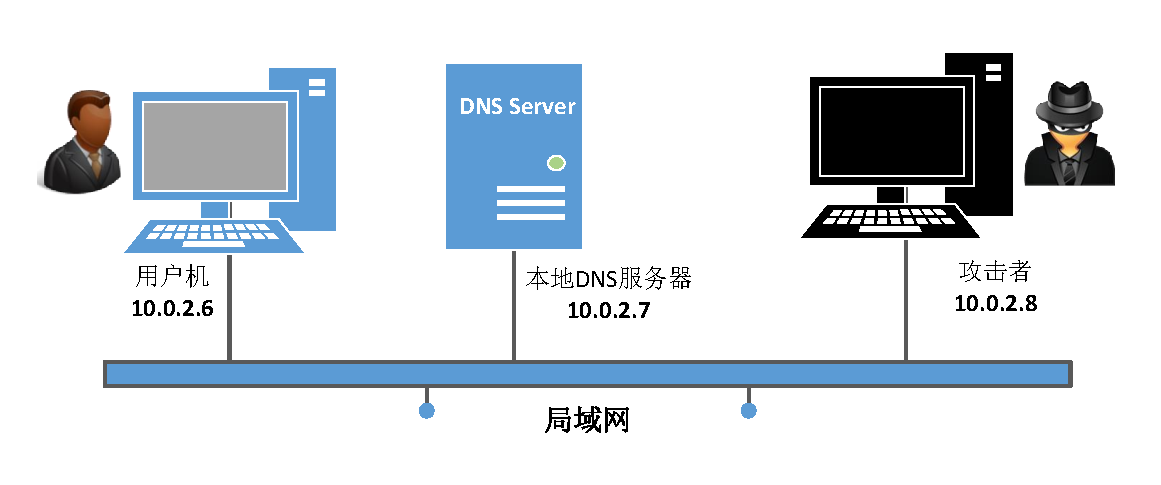
\includegraphics[width=0.9\textwidth]{\dnsFigs/environment_setup_remote.pdf}
\caption{实验环境搭建}
\label{dns:fig:environment}
\end{figure}


DNS缓存中毒攻击的主要目标是本地DNS服务器。显然,攻击真实的DNS服务器是违法的,因此
我们需要搭建自己的DNS服务器来进行攻击实验。本次实验环境需要三台主机:受害者主机,DNS服务器和
攻击者主机。我们在单个宿主机上运行这三个虚拟机,这些VMs都使用我们预先构建的\ubuntu VM镜像。
图~\ref{dns:fig:environment}说明了实验环境的设置。如果使用{\tt VirtualBox},请使用
{\tt "NAT Network"}作为每个VM的网络适配器选项,如果使用{\tt Vmware},使用默认的{\tt "NAT"}即可。
为了简单起见,我们将这些VMs都放在同一LAN中,学生不能在攻击中利用这个便利,他们应该将攻击者的机器
视为远程机器,即攻击者无法在LAN上嗅探数据包。


在以下各节中,我们假定用户计算机的IP地址为{\tt 10.0.2.6},本地DNS服务器的IP地址为{\tt 10.0.2.7},
攻击者主机的IP地址为{\tt 10.0.2.8},我们称本地DNS服务器为\texttt{Apollo}。



% -------------------------------------------
% SUBSECTION
% ------------------------------------------- 
\subsection{任务 1: 配置用户主机} 
\label{subsec:user_machine}


在用户主机{\tt 10.0.2.6}上,我们需要使用{\tt 10.0.2.7}作为本地的DNS服务器。
这是通过更改用户主机的解析配置文件~(\texttt{/etc/resolv.conf})来实现的,将
\texttt{10.0.2.7}添加为第一个\texttt{nameserver}条目,即该服务器将用作主DNS服务器。
然而,由于我们提供的VM都采用Dynamic Host Configuration Protocol (DHCP)来获取网络配置参数,例如IP地址,本地DNS服务器等,
DHCP 客户端会用从DHCP服务器获取的网络配置信息覆盖并重写\texttt{/etc/resolv.conf} 文件。


为防止我们在 \texttt{/etc/resolv.conf} 文件中的配置被DHCP覆盖,我们可以添加以下内容到
\path{/etc/resolvconf/resolv.conf.d/head}文件中(假设\texttt{10.0.2.7}是本地DNS服务器的IP地址):


\begin{lstlisting}
nameserver 10.0.2.7
\end{lstlisting}


Head文件的内容会加在自动生成的配置文件之前,通常来说只是一个注释行 ( \texttt{/etc/resolv.conf} 的注释往往来自其head文件 ) 。
在完成修改之后,我们需要执行以下命令来使修改生效:

\begin{lstlisting}
$ sudo resolvconf -u
\end{lstlisting}



\paragraph{测试:}

在成功配置完用户主机后,使用\texttt{dig}命令来尝试获取一个主机名(hostname)的IP地址,从dig的回显来查看
响应内容是否是从本地的DNS服务器返回,如果不是则证明未成功配置。



% -------------------------------------------
% SUBSECTION
% ------------------------------------------- 
\subsection{任务 2: 配置本地DNS服务器 (the Server VM)} 


针对本地DNS服务器,我们需要运行一个DNS服务软件,目前用的最广的DNS服务软件是BIND~(Berkeley Internet Name
Domain),该软件最初由加州大学伯克利分校于1980年代初期开发设计,最新的版本
名为BIND 9,它于2000年首次发布。我们将在实验环境下展示如何配置BIND 9软件。
BIND 9软件已经预装在\ubuntu VM镜像中并会在系统开启时自启动。


BIND 9 从配置文件\path{/etc/bind/named.conf}读入软件配置,该文件是主配置文件,
它通常包含许多\texttt{"include"}入口,真正的配置内容往往保存在这些引入文件中。
其中我们通常需要设置的是\path{/etc/bind/named.conf.options}文件:


\paragraph{Step 1:删除 {\tt example.com} 区域:}
如果你做了 ``本地DNS攻击实验'',你很有可能已经配置了本地DNS服务器{\tt Apollo}来管理
{\tt example.com}域。在本实验中,该DNS服务器不再管理这个域,因此需要从{\tt /etc/bind/named.conf}
文件中删除相关的域设置。



\paragraph{Step 2: 配置一个正向区域:}
在本实验中,Kaminsky攻击的主要目的是使受害者使用 \texttt{ns.attacker32.com} 作为
\texttt{example.com}域的名称服务器。一旦攻击成功,受害DNS服务器会将对\texttt{example.com}域
的所有查询发送给\texttt{ns.attacker32.com}。 



在现实世界中,当本地DNS服务器需要查找\texttt{ns.attacker32.com}的IP地址。
它将前往根服务器 \texttt{com}服务器询问,并最终从管理\texttt{attacker32.com}域的名称
服务器获得响应。一旦本地DNS服务器得到这个IP地址,它会向这个IP地址发查询请求。这也是学生
会遇到问题的地方,因为学生不拥有\texttt{attacker32.com}域名(该域名事实上由本实验的作者杜文亮教授拥有),
因此学生将无法配置运行在\texttt{ns.attacker32.com}域的DNS服务器。


为解决这一问题,学生可以购买自己的域名,并在攻击中使用自己购买的域名,而不是\texttt{attacker32.com}。
这样,学生可以自己配置他们的DNS服务器来进行回答响应。然而这种方法对于学生来说成本太高了。
 

幸运的是,BIND9允许我们在DNS配置中添加一个正向区域。将以下区域条目添加到\path{/etc/bind/named.conf}文件中。
这项条目表示对于\texttt{attacker32.com}域的所有查询,都将转发到\texttt{10.0.2.8}。
这等效于将\texttt{10.0.2.8}作为\texttt{attacker32.com}域的名称服务器。
因此,使用这个配置,本地DNS服务器不会去查询\texttt{attacker32.com}域的IP地址,因为它已经有IP地址了。
请不要忘记配置中的所有分号,不然配置会失效。


\begin{lstlisting}
zone "attacker32.com" {
    type forward;
    forwarders {
        10.0.2.8;
    };
};
\end{lstlisting}
 


\paragraph{Step 3: 配置一些选项:} 
在我们的SEED虚拟机中,我们已经完成了所有的配置,这里只是希望学生可以了解到我们所做的配置内容。
如果学生使用的是SEED VM,那么这里不需要做任何操作。我们完成的配置内容在 \path{/etc/bind/named.conf.options}文件中。


\begin{itemize} 
\item 
\textbf{配置DNS缓存的转储位置:} 
以下配置指定了当BIND需要转储DNS缓存时,缓存文件的存储位置。如果该选项没有指定,
BIND将转储缓存到默认文件\path{/var/cache/bind/named_dump.db}。

\begin{lstlisting}
  options {
      dump-file "/var/cache/bind/dump.db";
  };
\end{lstlisting}

下面两个命令与DNS缓存相关,第一个命令将DNS缓存内容转储到之前指定的位置,第二个命令将清除缓存。


\begin{lstlisting}
$ sudo rndc dumpdb -cache    // 转储DNS缓存到指定位置
$ sudo rndc flush            // 清除DNS缓存
\end{lstlisting}


\item 
\textbf{关闭 DNSSEC:} 
DNSSEC的引入为了防止DNS服务器受到欺骗攻击,
为了展示DNS攻击的效果,我们需要关闭这种保护机制。可以通过修改\path{named.conf.options}文件:
注释掉{\tt dnssec-validation} 行,添加一行
{\tt dnssec-enable} 。

\begin{lstlisting}
  options {
      # dnssec-validation auto;
      dnssec-enable no;
  };
\end{lstlisting}


\item 
\textbf{固定源端口号:}
DNS服务器现在在DNS查询中随机化源端口号,这使得攻击更加的困难。不幸的是,许多DNS服务器
仍然使用可以预测的源端口号。在本实验中,出于简单的考虑,我们假设源端口号是一个固定的数字。
我们可以将所有DNS请求的源端口设置为{\tt 33333}。可以通过在{\tt /etc/bind/named.conf.options}文件
中添加以下配置来生效:


\begin{lstlisting}
   query-source port 33333
\end{lstlisting}

\end{itemize}



\paragraph{Step 4: 重启DNS服务器:}
我们可以用以下命令重启DNS服务器。每次修改DNS配置后,DNS服务器都需要重启来使配置生效。
以下命令可以启动或重启\texttt{BIND 9}DNS服务器。

\begin{lstlisting}
$ sudo service bind9 restart
\end{lstlisting}




% -------------------------------------------
% SUBSECTION
% ------------------------------------------- 
\subsection{任务 3: 配置攻击者主机}

在攻击者主机,我们将管理两个区域。一个是攻击者合法的区域\texttt{attacker32.com},
另一个是假的\texttt{example.com}区域。


\begin{itemize} 
\item Step 1: 从实验网站下载\texttt{attacker32.com.zone}和
              \texttt{example.com.zone}文件。 

\item Step 2: 根据学生实际的网络配置修改这些文件(e.g., 一些IP地址需要修改)。 

\item Step 3: 将这两个文件拷贝到\texttt{/etc/bind} 目录。 

\item Step 4: 在\path{/etc/bind/named.conf}添加以下条目:


\begin{lstlisting}
zone "attacker32.com" {
        type master;
        file "/etc/bind/attacker32.com.zone";
};

zone "example.com" {
        type master;
        file "/etc/bind/example.com.zone";
};
\end{lstlisting}


\item Step 5: 重启DNS服务器。
\end{itemize} 
 


% -------------------------------------------
% SUBSECTION
% ------------------------------------------- 
\subsection{任务 4: 测试配置}

对于用户主机,我们运行一系列命令来确保我们的配置正确。


\paragraph{获取\texttt{ns.attacker32.com}的IP地址:}
当我们运行以下的\texttt{dig}命令时,由于在DNS配置中添加的\texttt{forward}区域,本地
DNS服务器会将查询请求转发到攻击者主机。因此,响应会从攻击者主机上配置的
\texttt{attacker32.com.zone}文件中返回。如果返回的结果不符合预期,那么配置过程可能存在问题。
请在实验报告中描述你的观察。


\begin{lstlisting}
$ dig ns.attacker32.com
\end{lstlisting}



\paragraph{获取\texttt{www.example.com}的IP地址:} 
目前有两个名称服务器管理\texttt{example.com}域,一个是这个域的官方名称服务器,另一个
是攻击者主机。我们将请求这两个名称服务器来查看会得到怎样的响应。
请运行以下两条命令(在用户主机上),并描述你观察到的现象。 


\begin{lstlisting}
// 发送请求到本地DNS服务器,这个请求会前往example.com的官方名称服务器
$ dig www.example.com

// 直接向ns.attacker32.com发送请求 
$ dig @ns.attacker32.com www.example.com
\end{lstlisting}
 


显然,没有人会向 \texttt{ns.attacker32.com}请求 \texttt{www.example.com}的IP地址,
人们会向 \texttt{example.com}域的官方名称服务器请求答案。所以DNS缓存攻击的目的是让
受害者去向\texttt{ns.attacker32.com}询问\texttt{www.example.com}的IP地址。顾名思义,
如果我们的攻击成功,当我们运行第一个\texttt{dig}命令时,即不带有 \texttt{@}选项的,我们应该
从攻击者主机得到一个虚假的结果,而不是从合法的名称服务器得到一个真实的结果。



% *******************************************
% SECTION
% ******************************************* 
\section{攻击任务}


DNS攻击的主要目的是在用户尝试使用$A$的域名前往$A$主机时,将用户重定向到另一个主机$B$。
例如,假设{\tt www.example.com}是一个在线银行网站,当用户尝试使用正确的URL {\tt www.example.com}
访问该网站时,如果攻击者可以将用户重定向到一个非常类似于{\tt www.example.com}的恶意站点,
那么用户很有可能被欺骗并向攻击者泄露自己的用户名密码。


在此任务中,我们将域名{\tt www.example.com}作为我们的攻击目标。值得注意的是, {\tt example.com}
域名保留供实验使用,不用作任何真实用途。 {\tt www.example.com}的真实IP地址为{\tt 93.184.216.34},
它的名称服务器由Internet Corporation for Assigned Names and Numbers (ICANN)管理。当用户
针对该域名运行{\tt dig}命令或在浏览器中输入该域名,用户主机会向本地DNS服务器发送DNS查询请求,
该DNS服务器最终将从{\tt example.com}的名称服务器中请求IP地址。


攻击的目标识对本地DNS服务器进行DNS缓存投毒攻击,例如当用户运行{\tt dig}命令来查找
{\tt www.example.com}的IP地址时,本地DNS服务器最终会进入攻击者的名称服务器{\tt ns.attacker32.com}
以获得IP地址,因此返回的IP地址可以是攻击者设计的任何值。结果,用户会被导向攻击者的恶意站点,而不是
真实的{\tt www.example.com}。




\begin{figure}[htb]
\centering
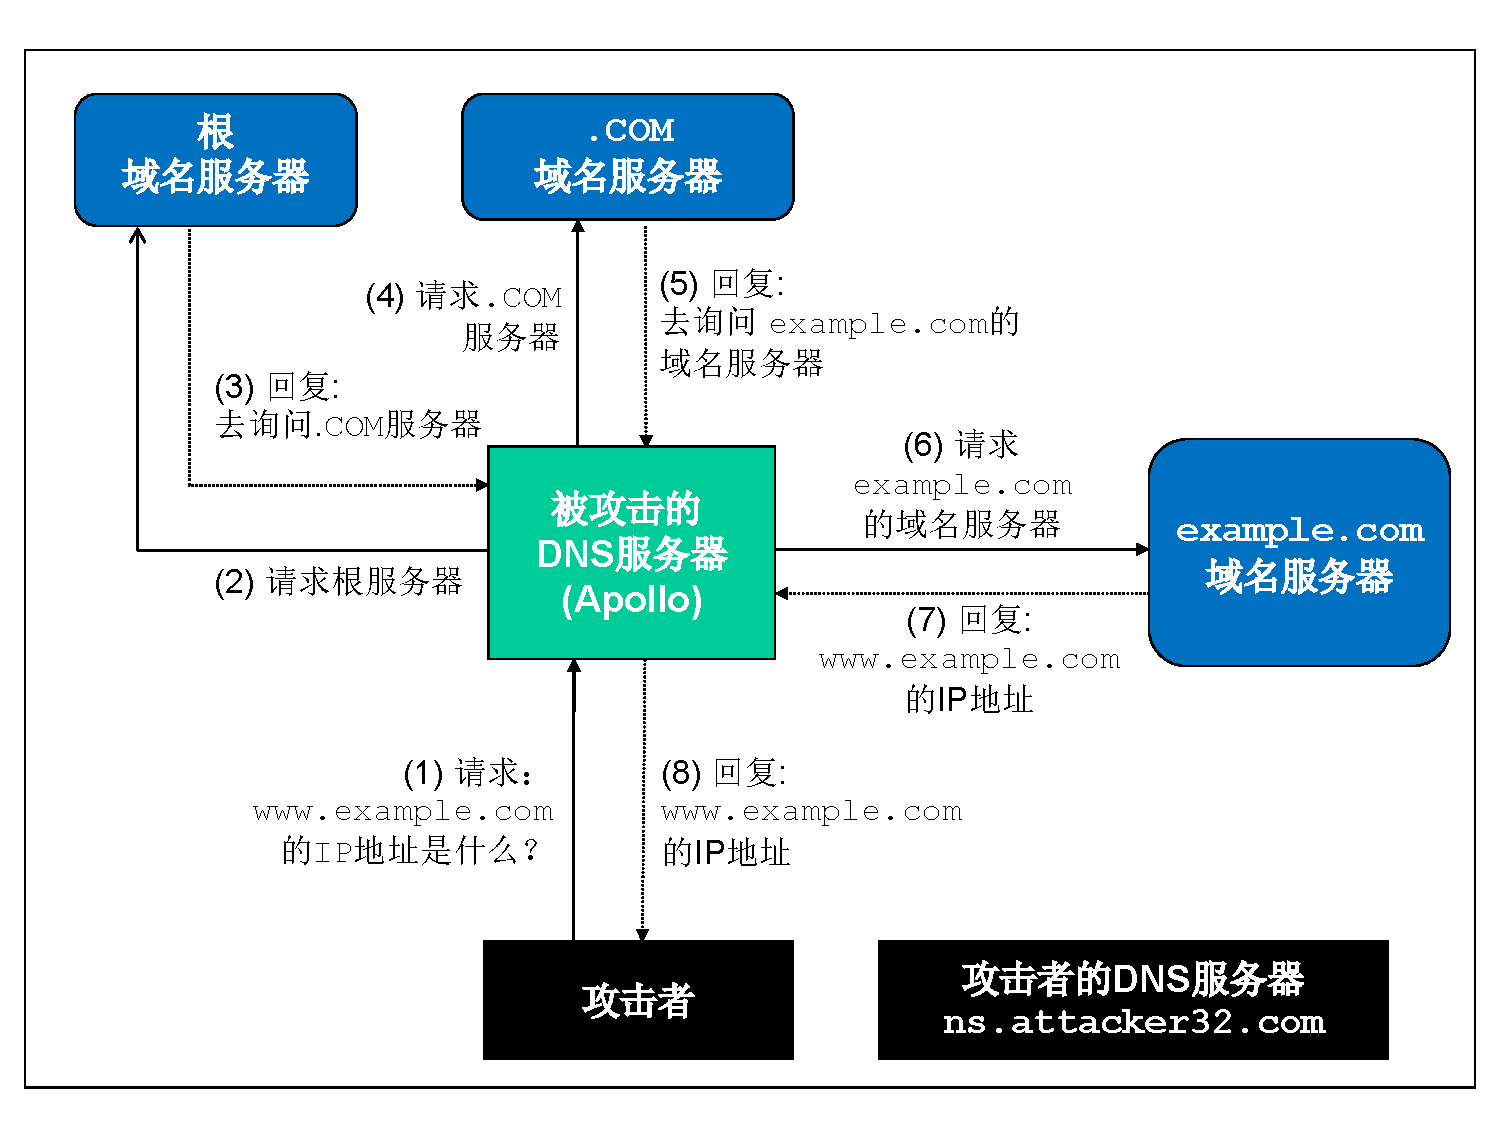
\includegraphics[width=0.9\textwidth]{\dnsFigs/DNS_Remote_new1.pdf}
\caption{完整的DNS查询过程} 
\label{fig:flow_diagram1}
\end{figure}


\begin{figure}[htb]
\centering
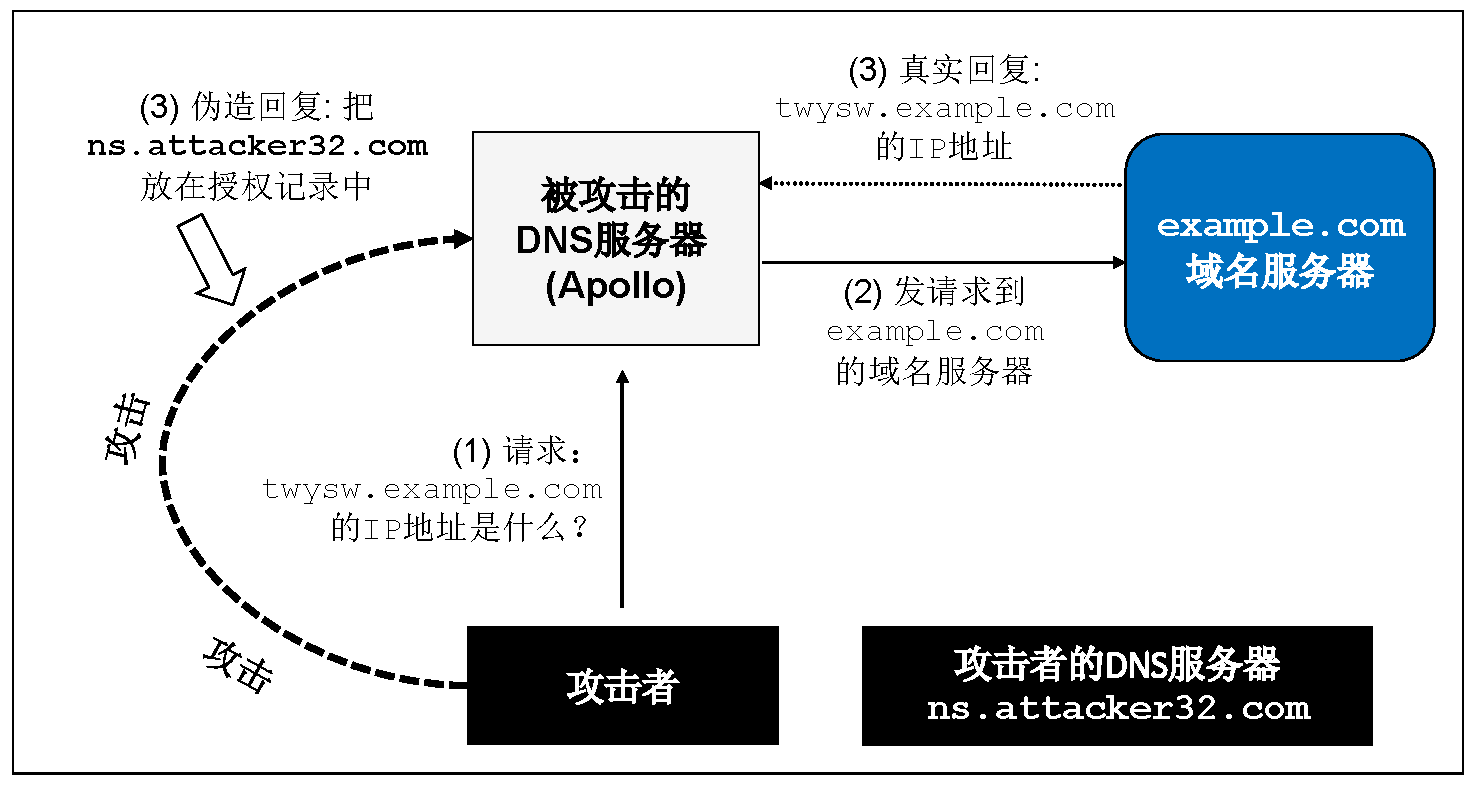
\includegraphics[width=0.9\textwidth]{\dnsFigs/DNS_Remote_new2.pdf}
\caption{Kaminsky攻击}
\label{fig:flow_diagram2}
\end{figure}



% -------------------------------------------
% SUBSECTION
% ------------------------------------------- 
\subsection{Kaminsky攻击原理}

在此任务中,攻击者向受害DNS服务器 ({\tt Apollo})发送DNS查询请求,从而触发来自
{\tt Apollo}的DNS查询。DNS查询首先前往其中一个根DNS服务器,接着 {\tt .COM}的DNS服务器,最终
从{\tt example.com}的DNS服务器得到查询结果,查询过程如图~\ref{fig:flow_diagram1}所示。
如果{\tt example.com}的名称服务器信息已经被{\tt Apollo}缓存,
那么查询不会前往根服务器以及{\tt .COM}DNS服务器,这个过程如图~\ref{fig:flow_diagram2}所示。
在本实验中,图~\ref{fig:flow_diagram2}描绘的场景更为常见,因此我们以这个图为基础来描述攻击机制。


当{\tt Apollo}等待来自{\tt example.com}名称服务器的DNS答复时,攻击者可以发送伪造的答复给{\tt Apollo},
假装这个答复是来自 {\tt example.com}的名称服务器。如果伪造的答复先到达,那么它将被
{\tt Apollo}接收,攻击成功。


如果你已经完成了本地DNS攻击的实验,你应该会意识到这些攻击都是假定攻击者和DNS服务器位于同一网段的,
即攻击者可以观察到DNS查询消息。当攻击者与DNS服务器不在同一网段,缓存投毒攻击变得非常困难。
主要的难点在于DNS响应中的传输ID(Transcation ID)必须与查询请求中的相匹配。由于查询中的传输ID
通常是随机生成的,在看不到请求包的情况下,攻击者很难猜到正确的传输ID。


显然,攻击者可以猜测传输ID。由于传输ID只有16位比特大小,如果攻击者可以在攻击窗口内伪造
$K$个响应(即在合法响应到达之前),那么攻击成功的可能性就是$K$/$2^{16}$。发送数百个伪造响应
并不是不切实际的,因此攻击者在成功之前不会进行太多的尝试。


然而,上述假设的攻击忽略了DNS缓存。在现实中,如果攻击者不幸没有在合法的响应到达之前猜中正确的传输ID,
那么DNS服务器会将正确的信息缓存一段时间。这种缓存效果使攻击者无法继续伪造针对该域名的响应,
因为DNS服务器在缓存超时之前不会针对该域名发出另一个DNS查询请求。为了继续对同一个域名的
响应伪造,攻击者必须等待针对该域名的另一个DNS查询请求,这意味着他必须要等到缓存超时。这个
等待时间可以是几小时或是几天。


\paragraph{Kaminsky攻击:} 
Dan Kaminsky提出了一个巧妙的方法来解决缓存的问题~\cite{dns:Kaminsky}。
通过他的方案,攻击者可以持续地发起欺骗攻击,而不需要等待,因此攻击可以在很短的
一段时间内成功。攻击的详细描述在~\cite{dns:Kaminsky,seedbook}可以找到。
在本任务中,我们将尝试这个攻击手段。以下步骤参考图~\ref{fig:flow_diagram2}概述了攻击的过程。


\begin{enumerate}
\item 攻击者向DNS服务器{\tt Apollo} 请求{\tt example.com}域中不存在的子域名,
如{\tt twysw.example.com},其中{\tt twysw}是一个随机的名字。 

\item 由于在{\tt Apollo}的DNS缓存中不可能匹配到这个子域名,因此{\tt Apollo} 
向{\tt example.com}域的名称服务器发送一个DNS查询请求。

\item 当{\tt Apollo} 等待答复时,攻击者向 {\tt Apollo}发送大量的伪造的DNS响应,
每个响应尝试一个不同的传输ID,希望其中一个是正确的。在响应中,攻击者不仅提供{\tt twysw.example.com}的
IP地址解析,攻击者还提供了一条``权威授权服务器''记录,其中指明{\tt ns.attacker32.com}是
{\tt example.com}域的名称服务器。如果伪造的响应比实际响应到达的早,且传输ID与请求中传输ID相匹配,
{\tt Apollo}就会接受并缓存伪造的答案,进而{\tt Apollo}的DNS缓存被投毒了。

\item 即使伪造的DNS响应失败了(例如,传输ID不匹配或到达的太晚了),
也没有关系,因为下一次攻击者会请求另一个子域名,所以{\tt Apollo}会发送另一个DNS请求,
从而给攻击者提供了另一个机会进行欺骗攻击。这种方法有效地克服了DNS缓存效果。



\item 如果攻击成功,那么在{\tt Apollo}的DNS缓存中,
{\tt example.com}域的名称服务器会被攻击者替换成{\tt ns.attacker32.com}。
为显示攻击的成功,学生需要展示在{\tt Apollo}的DNS缓存中有这样一条记录。
 


\end{enumerate}


\paragraph{任务综述:} 实现Kaminsky攻击十分具有挑战,因此我们将它分解为好几个子任务。在
任务4中,我们构造一个针对\texttt{example.com}域的随机子域名的DNS查询请求;在任务5中,我们构造一个从 \texttt{example.com}
名称服务器返回的伪造响应;在任务6中,我们把这些合在一起进行Kaminsky攻击;最后在任务7中我们验证攻击的效果。


% -------------------------------------------
% SUBSECTION
% ------------------------------------------- 
\subsection{任务 4: 构造DNS请求} 

这任务着重发送DNS请求。为了完成攻击,攻击者需要触发目标DNS服务器发出DNS查询,这样攻击者
有机会去欺骗DNS响应。由于攻击者需要尝试多次才能成功,因此最好使用程序来自动化该过程。

学生需要编写一个程序来向目标服务器发送DNS请求(即我们配置的本地DNS服务器)。学生的任务是
编写该程序并证明(使用Wireshark)他们的查询请求可以触发目标DNS服务器会发出相应的DNS查询。
该任务对性能的要求不高,因此学生可以使用C语言或Python(使用Scapy)编写此代码。以下提供了
Python的代码示例(其中\texttt{+++}是占位符,学生需要将他们替换为实际的值):


\begin{lstlisting}
Qdsec  = DNSQR(qname='www.example.com')
dns    = DNS(id=0xAAAA, qr=0, qdcount=1, ancount=0, nscount=0,
             arcount=0, qd=Qdsec)

ip  = IP(dst='+++', src='+++')
udp = UDP(dport=+++, sport=+++, chksum=0)
request = ip/udp/dns
\end{lstlisting}
 

\paragraph{Scapy:} 如果你使用Python3,那么在SEED VM中可能没有预先安装Scapy,你需要使用
一下命令安装Python3的Scapy包。


\begin{lstlisting}
$ sudo pip3 install scapy
\end{lstlisting}
 

% -------------------------------------------
% SUBSECTION
% ------------------------------------------- 
\subsection{任务 5: 伪造DNS响应}   

在此任务中,我们需要伪造Kaminsky攻击中的DNS响应。由于我们的攻击目标是\texttt{example.com},
我们需要欺骗从该域的名称服务器返回的响应。学生首先需要找到\texttt{example.com}域的合法名称服务器
的IP地址(值得注意的是这个域名有许多名称服务器)。

学生可以使用Scapy来实现这个任务,以下的代码示例构建了一个DNS响应包,其中包含了问题部分,
回答部分以及一个名称服务器部分。在这段代码中,我们使用\texttt{+++}作为占位符,学生
需要用Kaminsky攻击中所需要的值来替换。学生需要解释为什么选择这些值。

\begin{lstlisting}
name   = '+++'  
domain = '+++'  
ns     = '+++'

Qdsec  = DNSQR(qname=name)
Anssec = DNSRR(rrname=name,   type='A',  rdata='1.2.3.4', ttl=259200)
NSsec  = DNSRR(rrname=domain, type='NS', rdata=ns, ttl=259200)
dns    = DNS(id=0xAAAA, aa=1, rd=1, qr=1,
             qdcount=1, ancount=1, nscount=1, arcount=0,
             qd=Qdsec, an=Anssec, ns=NSsec)

ip    = IP(dst='+++', src='+++')
udp   = UDP(dport=+++, sport=+++, chksum=0)
reply = ip/udp/dns
\end{lstlisting}
 

由于这些响应本身无法进行成功的攻击,为了展示这个任务的效果,学生需要使用Wireshark来
捕获伪造的DNS响应,并证明伪造包是合法的。



% -------------------------------------------
% SUBSECTION
% ------------------------------------------- 
\subsection{任务 6: 进行Kaminsky攻击}   

现在我们将所有东西合在一起进行Kaminsky攻击。在攻击中,我们需要发送许多欺骗的DNS响应,
希望其中有一个可以猜中正确的传输ID并比合法的响应更早到达。因此,发包速度至关重要:我们能
发出越多的数据包,我们的成功率也就越高。如果我们使用Scapy来发送DNS响应包就如在之前的任务那样,
那么成功率将非常低。学生可以使用C语言进行实现,但在C语言中构造DNS数据包并非易事。
因此我们引入了使用C语言和Scapy相结合的混合方法。


通过混合方法,我们首先使用Scapy生成DNS数据包模板,并把模板保存在文件中。
接着我们将该数据包模板加载到C程序中,并对其中某些字段进行一些微小修改,然后发出这个数据包。
我们在实验网站提供了C语言的代码框架 (\texttt{attack.c})。
学生可以对其中标记的区域进行修改,详细的代码解释在之后的指南部分中。



\paragraph{检查DNS缓存:}
为了检查攻击是否成功,我们需要查看{\tt dump.db}文件来检查伪造的DNS响应是否成功被DNS服务器接收。
以下的命令行脚本可以转储DNS缓存,并搜索缓存中是否存在\texttt{attacker}字词(在我们的攻击中,我们
采用\texttt{attacker32.com}作为攻击者的域名,如果学生使用不同的攻击域名,那么需要搜索不同的字词)。
 

\begin{lstlisting}
#!/bin/bash

sudo rndc dumpdb -cache
cat /var/cache/bind/dump.db | grep attacker
\end{lstlisting}
 

% -------------------------------------------
% SUBSECTION
% ------------------------------------------- 
\subsection{任务 7: 攻击结果验证}

如果攻击成功,在本地DNS服务器的缓存中,\texttt{example.com}的{\tt NS}记录应该会改为
\texttt{ns.attacker32.com}。当服务器收到对\texttt{example.com}域内的任何子域名的解析请求时,
它会向\texttt{ns.attacker32.com}发送查询请求,而不是原本合法的名称服务器。


为了验证攻击是否成功,在用户主机上运行以下两条\texttt{dig}命令。在两个响应中,
\texttt{www.example.com}的IP地址应该相同,并且响应应该是在攻击主机的区域文件中配置的内容。


\begin{lstlisting}
// 询问本地DNS服务器来进行查询
$ dig www.example.com

// 直接请求attacker32名称服务器
$ dig @ns.attacker32.com www.example.com
\end{lstlisting}
 
请在实验报告中给出你的观察结果(截图),并解释你认为攻击成功的原因。
特别的,当你第一次运行\texttt{dig}命令时,请使用Wireshark来捕获网络流量,
并指出\texttt{dig}命令触发了哪些数据包。根据数据包追踪来证明你的攻击成功了。





% *******************************************
% SECTION
% ******************************************* 
\section{指南} 

为了实现Kaminsky攻击,我们使用Scapy进行数据包欺骗。不幸的是,Python的速度太慢了,Python每秒
生成的数据包太少以至于很难攻击成功。最好的情况是使用C程序,然而这对于许多学生来说颇具挑战,
因为用C构造DNS数据包并非易事。我们开发了一种混合方法,并在课堂上进行了实验。通过这种方法,
可以大大减少学生在编码上花费的时间,因此他们可以将更多的时间用于关注实际攻击的本身。


这个想法是同时利用Scapy和C的优势:Scapy在构建DNS数据包方便比C更方便,但是C速度更快。
因此我们使用Scapy构建伪造的DNS数据包,并将它保存到文件中,接着我们将数据包加载到C程序中。
尽管在Kaminsky攻击过程中,我们需要发送许多不同的DNS数据包,但除了少数字段外,这些数据包几乎相同。
我们可以将Scapy生成的数据包作为基础,找到需要修改地方的偏移量(如传输ID字段),并直接进行修改。
这比在C中创建整个DNS数据包要简单很多。
进行修改之后,我们使用原始的套接字发送这些数据包。有关这种混合方法的详细信息,请参见SEED书~\cite{seedbook}中
``数据包嗅探和伪造''一章。以下的Scapy程序会创建一个简单的DNS响应数据包,并将其保存在文件中。


\begin{lstlisting}[caption={\texttt{generate\_dns\_reply.py}}]
#!/usr/bin/python3
from scapy.all import *

# 构造DNS头和内容
name   = 'twysw.example.com'
Qdsec  = DNSQR(qname=name)
Anssec = DNSRR(rrname=name, type='A', rdata='1.1.2.2', ttl=259200)
dns    = DNS(id=0xAAAA, aa=1, rd=0, qr=1, 
             qdcount=1, ancount=1, nscount=0, arcount=0, 
             qd=Qdsec, an=Anssec)

# 构造IP、UDP头以及完整的数据包
ip  = IP(dst='10.0.2.7', src='1.2.3.4', chksum=0)
udp = UDP(dport=33333, sport=53, chksum=0)
pkt = ip/udp/dns

# 保存数据包到文件
with open('ip.bin', 'wb') as f:
  f.write(bytes(pkt))
\end{lstlisting}

在C程序中,我们从文件\texttt{ip.bin}中读入数据包,并将其用作数据包的模板,在此模板上,
我们可以创建许多类似的数据包,并向本地DNS服务器发送这些欺骗包。对于每个答复,我们修改
三个位置:传输ID和在两个位置(询问部分和回答部分)出现的的\texttt{twysw}。传输ID是一个固定的
位置(从IP数据包开头偏移\texttt{28}),但名称\texttt{twysw}的偏移位置取决于域名的长度。
我们可以使用二进制编辑器,如\texttt{bless},来查看二进制文件\texttt{ip.bin}并找到
\texttt{twysw}的两个偏移量。在我们的数据包中,他们的偏移是\texttt{41} 和 \texttt{64}。


以下的代码片段显示了我们如何修改这些字段。我们将响应中的域名改为\texttt{bbbbb.example.com},
并发出一个伪造的DNS答复(传输ID为\texttt{1000})。
在代码中,变量\texttt{ip}指向IP数据包的起始点。
 

\begin{lstlisting}
  // 修改询问字段的域名 (offset=41)
  memcpy(ip+41, "bbbbb" , 5);

  // 修改回答字段的域名 (offset=64)
  memcpy(ip+64, "bbbbb" , 5);

  // 修改传输ID字段 (offset=28)
  unsigned short id = 1000;
  unsigned short id_net_order = htons(id);
  memcpy(ip+28, &id_net_order, 2);
\end{lstlisting}



\paragraph{生成随机子域名:} 在Kaminsky攻击中,我们需要生成随机的子域名。
有许多方法可以做到这一点。以下的代码片段展示了如何生成一个5个字符的随机子域名。


\begin{lstlisting}
char a[26]="abcdefghijklmnopqrstuvwxyz";

// 生成一个长度为5的随机子域名
char name[5];
for (int k=0; k<5; k++)  
   name[k] = a[rand() % 26];
\end{lstlisting}
 



% *******************************************
% SECTION
% ******************************************* 
\section{Submission}

\seedsubmission


%%%%%%%%%%%%%%%%%%%%%%%%%%%%%%%%%%%%%%%%%%
\thispagestyle{empty}
\bibliographystyle{plain}
\def\baselinestretch{1}
\bibliography{BibDNS}
%%%%%%%%%%%%%%%%%%%%%%%%%%%%%%%%%%%%%%%%%%



\end{document}
%%%%%%%%%%%%%%%%%%%%%%%%%%%%%%%%%%%%%%%%%%%
%%%%%%%%%%%%%%%%%%%%%%%%%%%%%%%%%%%%%%%%%%%
%%%%%%%%%%%%%%%%%%%%%%%%%%%%%%%%%%%%%%%%%%%
%%%%%%%%%%%%%%%%%%%%%%%%%%%%%%%%%%%%%%%%%%%
%%%%%%%%%%%%%%%%%%%%%%%%%%%%%%%%%%%%%%%%%%%
%%%%%%%%%%%%%%%%%%%%%%%%%%%%%%%%%%%%%%%%%%%
%%%%%%%%%%%%%%%%%%%%%%%%%%%%%%%%%%%%%%%%%%%



